\section{Замеры}

\subsection{$U = 1$}
Для вычислений я сгенерировал по 1000 реплик длины 250, 500, 1000, 2000. При моделировании методом Монте-Карло делал 100000--300000 шагов на отжиг, и 500000--1000000 шагов для замеров. 
Оказалось что достаточно большая часть этих конформаций неплотные, то есть их свойства ближе к свойствам одномерной решётки, чем двумерной. При попытке посчитать среднее значения кумулянта Биндера неплотные конформации Сильно влияли на значение кумулянта, увеличивая погрешность от реплики к реплике.

\begin{figure}[h]
	\centering
	\begin{subfigure}[t]{0.48\textwidth}
		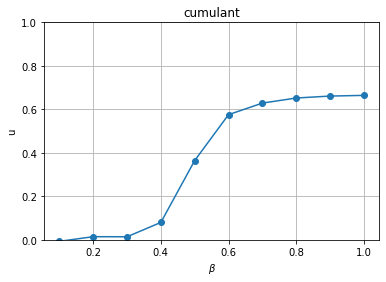
\includegraphics[width=\textwidth]{../images/dense_cumulant.png} 
		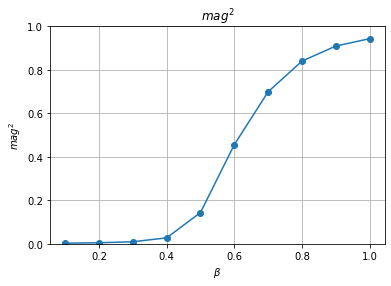
\includegraphics[width=\textwidth]{../images/dense_magnetization.png} 
		\caption{Плотная}
	\end{subfigure}
	\begin{subfigure}[t]{0.48\textwidth}
		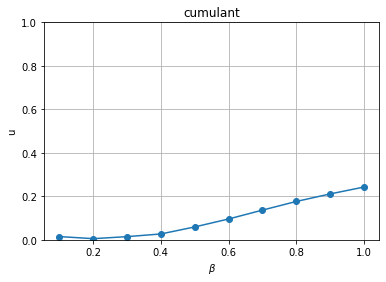
\includegraphics[width=\textwidth]{../images/loose_cumulant.png} 
		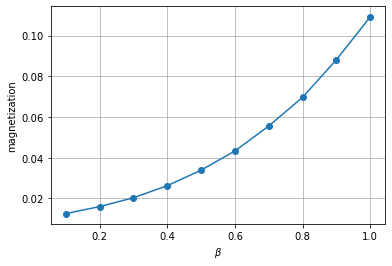
\includegraphics[width=\textwidth]{../images/loose_magnetization.png} 
		\caption{Неплотная}
	\end{subfigure}
	\caption{Пример кумулянта и намагниченности плотной и неплотной конформаций}
\end{figure}


\subsubsection{Разделение конформаций}

Для отделения плотных конформаций от остальных было предложено вычислять их радиус инерции.$R = \sqrt{\frac{1}{n}\sum_{i=1}^{n}r_{i}^{2}}$, где $r_i$ это расстояние от узла конформации до её центра масс. Однако при рассмотрении большого количества конформаций оказалось, что маленький радиус инерции не гарантирует хорошую намагниченность конформации

\begin{figure}[h]
	\centering
	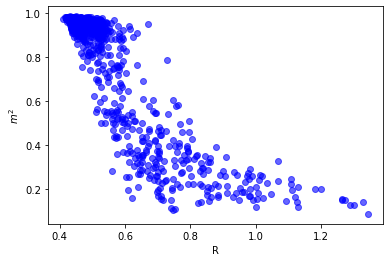
\includegraphics[width=\textwidth]{../images/mag2_to_R_L250.png} 
	\caption{Корреляция намагниченности конформаций при $\beta = 1$ и радиуса инерции для конформаций длины $L = 250$}
	\label{fig:mag2_to_R} 
\end{figure}

На рис.\ref{fig:mag2_to_R}, при $R \approx 0.6$ $m^2$ принимают любые значения от 0.2 до 1.0. Значит, при разделении конформации только по радиусу инерции, мы либо будем отбрасывать намагничивающиеся конформации, либо оставлять не намагничивающиеся

\paragraph{Кластеризованные конформации}

\begin{figure}[h!]
	\centering
	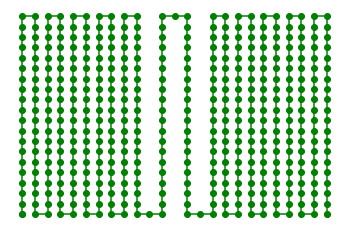
\includegraphics[width=0.47\textwidth]{../images/2Cluster_conformation.png}
	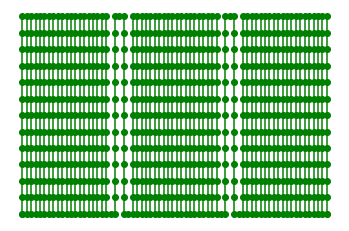
\includegraphics[width=0.47\textwidth]{../images/3Cluster_conformation.png} 
	\caption{Пример плотной немагнитной конформации}
	\label{fig:synth_cluster_conf}
\end{figure}

На искусственном примере рис.\ref{fig:synth_cluster_conf} показана одна из причин, по которой плотная конформация может плохо намагничиваться. Тут имеется несколько крупных двумерных кластеров, соединённых одномерной цепочкой. И не смотря на то, что сами по себе эти кластеры намагничиваются, направление спинов в них слабо связано, из-за чего спины в разных кластерах с большой вероятностью будут направлены в противоположные стороны.


Следующей задачей стало проанализировать конформации на количество и размеры кластеров, а так же мостов(одномерных сегментов) которые и соединяют. Первым вариантом было искать классические мосты -- спины, при удалении увеличивается число компонент связанности. Однако такой способ не дал желаемого эффекта, так как кластеры могут быть соединены более чем одним мостом. И например на конформации из рис. \ref{fig:clusters_and_bridges} данный способ не выделяет ни одного моста. 


Следующим вариантом стал данный алгоритм:

\begin{enumerate}
	\item Отметить все спины с 1 или 2 соседями как мосты.
	\item Убрать отметки со спинов, среди соседей которых есть не отмеченные спины.
	\item Создаём массив, где отмечаем посещённые спины, изначально все спины не посещены.
	\item Запускаем DFS(поиск в глубину) из не посещённого спина, который не является мостом.
	\item В DFS увеличиваем счётчик размера текущего кластера на 1, и запускаем DFS во всех соседях текущего спина, которые мы ещё не посетили и которые не помечены как мосты.
	\item Когда DFS посетил всех возможных соседей, получаем размер данного кластера.
	\item Повторяем пункты 4--6 пока не посетим все спины, не являющиеся мостами.
	\item Для определения размера и количества мостов делаем всё по аналогии с пунктами 4--7.
\end{enumerate}

\ref{fig:clusters_and_bridges}

\begin{figure}[h]
	\centering
	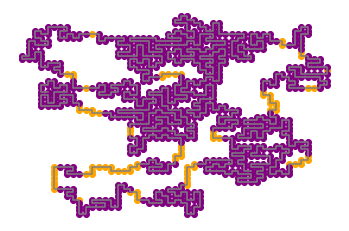
\includegraphics[width=0.47\textwidth]{../images/bridges_example_1.png}  
	\caption{Пример реальных конформаций с маленьким радиусом инерции и маленькой намагниченностью, с отмеченными мостами}
	\label{fig:claters_and_bridges}
\end{figure}




\subsection{Кумулянт и точка перехода}

Кумулянт Биндера для одной реплики при заданной температуре вычисляется по формуле $U = 1 - \frac{\langle m^4\rangle}{3\langle m^2\rangle ^2}$. Дальше Значения усредняются между репликами при каждой температуре $\langle U\rangle = \frac{1}{n}\sum_{i=1}^{n}U_i$ 
Погрешность кумулянта от реплики к реплике вычисляется как среднеквадратичное отклонение по формуле $\sqrt{\frac{1}{n}\sum_{i=1}^{n}(\langle U\rangle - U_i)^2}$


Если отбросить достаточное количество неплотных конформаций, то посчитав кумулянт по оставшимся можно увидеть точку перехода.

\begin{figure}[h]
	\centering
	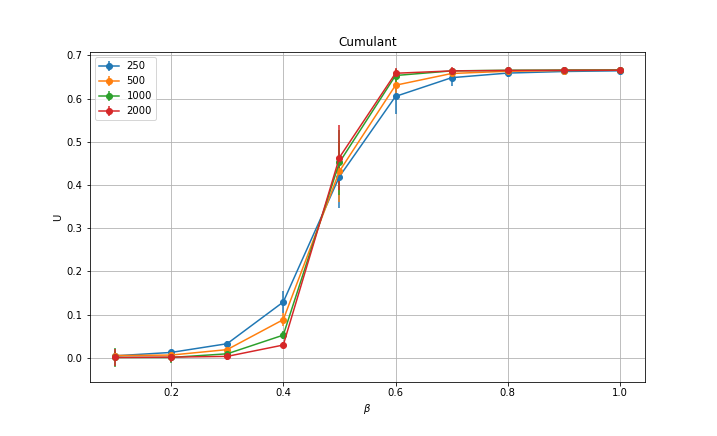
\includegraphics[width=1\textwidth]{../images/Cumulant_big.png} 
	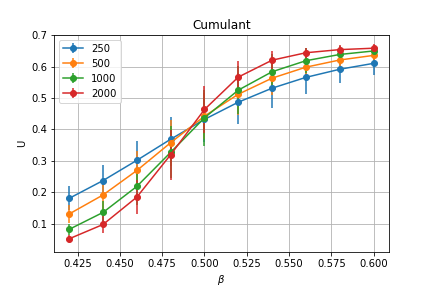
\includegraphics[width=1\textwidth]{../images/Cumulant_beta0.4_0.6.png} 
	\caption{Значения куулянтов после отбрасывания конформаций по радиусам}
\end{figure}
